%%% In this section, you will describe all of the various artifacts that you will generate and maintain during the project life cycle. Describe the purpose of each item below, how the content will be generated, where it will be stored, how often it will be updated, etc. Replace the default text for each section with your own description. Reword this paragraph as appropriate.

\subsection{Major Documentation Deliverables}

\subsubsection{Project Charter}
This document will be updated every sprint to reflect any changes the project may encounter. The changes may include: additional equipment/expenditures, added/removed functionality, etc. The initial version of this charter will be delivered Monday, October 1st and the final version will be delivered at the end of Senior Design II along with the final product.

\subsubsection{System Requirements Specification}
Describe how this document will be maintained and updated (how often, under what circumstances, etc.). When will the initial version be delivered? When will the final version be delivered?

\subsubsection{Architectural Design Specification}
Describe how this document will be maintained and updated (how often, under what circumstances, etc.). When will the initial version be delivered? When will the final version be delivered?

\subsubsection{Detailed Design Specification}
Describe how this document will be maintained and updated (how often, under what circumstances, etc.). When will the initial version be delivered? When will the final version be delivered?

\subsection{Recurring Sprint Items}

\subsubsection{Product Backlog}
Items from the SRS will be added to the product backlog based on how the overall architecture of the app is laid out. For example, requirements dealing with interfacing with the Octoprint and Google voice API would be some of the first items to be added to the backlog. These decisions will be decided by a group vote and the backlog will be maintained/shared on ----------???

\subsubsection{Sprint Planning}
In each sprint, the whole team will take around 1 hour per week for meeting to discuss about the next sprint. During the meeting, they will agree to complete a numbers of items of product backlog in the next sprint. Based on that, a sprint backlog is defined. This is how each sprint plan is planned. After looking at the schedules for this course and previous Senior Design II courses during the appropriate semesters, there will be 8 sprints (4 sprints for Senior Design I and 4 sprints for Senior Design II).

\subsubsection{Sprint Goal}
The Scrum Team will decide the sprint goal. Based on the customer's requirements, the Product Owner will list the objectives that the sprint should achieve. Based on that, the Scrum Team will decide the sprint goal. Then, the Development Team will select the Product Backlog Items that help to meet the sprint goal. 

\subsubsection{Sprint Backlog}
The Development Team decides which product backlog items make their way into the sprint backlog. The backlog will be maintained by scrum sprint Excel tool.

\subsubsection{Task Breakdown}
Individual tasks from the sprint backlog can be assigned in 2 ways: 
\begin{itemize}

\item If the level of difficulty of each task is the same, each member can voluntarily claim a task.

\item If the level of difficulty of each task is different, depend on the level and the ability of each member, each member must only assign the suitable tasks.  

\end{itemize}
Depending on the end date of each sprint, team members can estimate the time they think they will need to work on the tasks. Note: their estimated time must be as earlier as possible than the end date. 

\subsubsection{Sprint Burn Down Charts}
For each sprint, team members will keep updating the "Status" column for their assigned tasks. As long as the "Status" column is updated to "Finished", the sprint burn down chart will be updated and generated automatically. 

The total amount of effort expended by each individual team member can be accessed by:

\begin{itemize}
    
\item In each sprint backlog, looking for the "Assigned to" column to assign tasks for each member and checking on the "Status" column to know which task has been completed. 
Note: The "Assigned to" column lets you know which task each member works on.

\end{itemize}

The format of the sprint burn down chart is release burn down chart.

An example of the sprint burn down chart as below:

\begin{figure}[h!]
	\centering
   	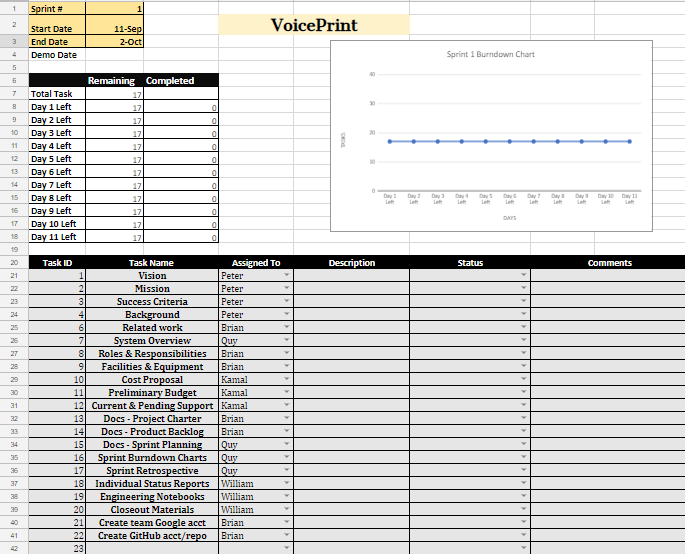
\includegraphics[width=0.6\textwidth]{images/Chart.png}
    \caption{Example sprint burn down chart}
\end{figure}

\subsubsection{Sprint Retrospective}
For each sprint, with the presentation of all team members, the team will firstly schedule a sprint review, then the team will schedule a sprint retrospective. The team will choose the time that is best fit for all team members. If the sprint review was good, the team would have discussion about sprint retrospective. Each task will be documented as individuals. After the group reviewing, all the tasks will be putting together as a single document before turning in as group. Each team has different due day for team assignment. In our team, we decide to have everything get done at least 3 days before the due day of the sprint.

\subsubsection{Individual Status Reports}
For every sprint, all group members will submit an individual status report. This report will show an individual's status on a given sprint (behind, ahead, etc). Some key items included in the status report include: the sprint goal, backlog, logged hours, burnout chart, and individual retrospective.

\subsubsection{Engineering Notebooks}
The engineering notebooks will be updated once a week at a minimum by each team member and each update will consist of one page. To maintain accountability, the team will meet before and/or after class every Monday and Wednesday. Currently the team plans on having no designated "witness" for the notebooks; therefore, the "witness" for each engineering notebook page will vary based on who was present when the notebook was being updated.

\subsection{Closeout Materials}

\subsubsection{System Prototype}
What will be included in the final system prototype? How and when will this be demonstrated? Will there be a Prototype Acceptance Test (PAT) with your customer? Will anything be demonstrated off-site? If so, will there be a Field Acceptance Test (FAT)?

\subsubsection{Project Poster}
What will be included on the poster, what will be the final dimensions, and when will it be delivered?

\subsubsection{Web Page}
What will be included on the project web page? Will it be accessible to the public? When will this be delivered? Will it be updated throughout the project, or just provided at closeout (at a minimum, you need to provide a simple web page at the end).

\subsubsection{Demo Video}
The demo videos will show how the app works. The video will show step-by-step how the app operates, beginning from the setup and ending with a finished 3D printed object. The video will be at most 5 minutes.

\subsubsection{Source Code}
How will your source code be maintained? What version control system will you adopt? Will source code be provided to the customer, or binaries only? If source code is provided, how will it be turned over to the customer? Will the project be open sourced to the general public? If so, what are the license terms (GNU, GPL, MIT, etc.). Where will the license terms be listed (in each source file, in a single readme file, etc.).

\subsubsection{Source Code Documentation}
What documentation standards will be employed? Will you use tools to generate the documentation (Doxygen, Javadocs, etc.). In what format will the final documentation be provided (PDF, browsable HTML, etc.)?

\subsubsection{Hardware Schematics}

\subsubsection{CAD files}

\subsubsection{Installation Scripts}
How will the customer deploy software to new installations? Will you provide installation scripts, install programs, or any other tools to improve the process? Will there be multiple scripts provided (perhaps separate scripts for the graphical front end and back end server software)? 

\subsubsection{User Manual}
A user manual will be provided in the app displayed as a help button. Setup as well as instructions on how to operate the app will be located here.
